\section{Planificación del Sprint 3}

\subsection{Descripción y fechas}
El Sprint 3 se desarrolló del 4 al 25 de noviembre de 2026. El equipo completó el flujo desde el registro de un certificado SIHA hasta el análisis, la revisión de los docentes y la decisión final cuando no hay acuerdo.

\subsection{Propósito y objetivos}
El propósito fue entregar una homologación explicable y revisable, con datos oficiales de la UTA y atención a los trámites externos. Se planificó registrar y revisar certificados, analizar las materias con el agente, aclarar el uso del mínimo del 80~\%, permitir los votos docentes y la decisión administrativa, guardar resultados por materia e incorporar registro manual y mejoras de cuentas.

\subsection{Análisis de capacidad}
Las horas de la tabla son la suma de las estimaciones de las tareas de código identificadas en los commits del período. No incluyen actividades sin un commit que las respalde.

\begin{table}[H]\centering\small
\begin{tabularx}{\textwidth}{|X|X|c|}\hline
\rowcolor{grisTarjeta}\textbf{Integrante} & \textbf{Rol en el sprint} & \textbf{Horas de tareas}\\\hline
Alex Jonathan Chisag & Frontend e integración & 57 h\\\hline
Rolando Sebastián Miranda & Backend, integración y pruebas & 58 h\\\hline
Jair León & Backend y correcciones & 15 h\\\hline
Paul Acurio & sin tareas de código registradas en el Sprint 3 & 0 h\\\hline
\textbf{Total registrado} & & \textbf{130 h}\\\hline
\end{tabularx}\caption{Capacidad de trabajo registrada en el Sprint 3}
\end{table}

\subsection{Product Backlog actualizado}
Las historias HU-01 a HU-06 del Sprint 1 están terminadas. Las HU-07 a HU-11 del Sprint 2 están terminadas con las correcciones descritas en la sección 7. El Sprint 3 tomó las historias HU-12 a HU-19, enfocadas en el certificado SIHA, el análisis, las decisiones y la operación del sistema.

\subsection{Sprint Backlog}
\begin{table}[H]\centering\small
\begin{tabularx}{\textwidth}{|c|X|X|c|c|c|}\hline
\rowcolor{grisTarjeta}\textbf{HU} & \textbf{Historia} & \textbf{Responsables con commits} & \textbf{SP} & \textbf{Horas} & \textbf{Prioridad}\\\hline
HU-12 & Registrar solicitud con certificado único y revisar antes del envío & Alex Jonathan Chisag; Jair León; Rolando Sebastián Miranda & 8 & 43 & Alta\\\hline
HU-13 & Analizar con sílabos oficiales y explicar cada materia & Rolando Sebastián Miranda; Alex Jonathan Chisag & 8 & 26 & Alta\\\hline
HU-14 & Comparar sílabo de otra universidad & Alex Jonathan Chisag & 5 & 4 & Media\\\hline
HU-15 & Aplicar la regla de créditos y contenidos del 80~\% & Alex Jonathan Chisag; Rolando Sebastián Miranda & 8 & 24 & Alta\\\hline
HU-16 & Registrar votos docentes y decisión final del administrador & Alex Jonathan Chisag; Rolando Sebastián Miranda & 8 & 14 & Alta\\\hline
HU-17 & Guardar el resultado de homologación por materia & Alex Jonathan Chisag & 5 & 4 & Media\\\hline
HU-18 & Registrar manualmente y sugerir solo materias relacionadas & Rolando Sebastián Miranda; Jair León & 5 & 11 & Media\\\hline
HU-19 & Administrar cuentas y avisar sobre la sesión & Alex Jonathan Chisag & 5 & 4 & Media\\\hline
\textbf{Total} & & & \textbf{52} & \textbf{130} & \\\hline
\end{tabularx}\caption{Sprint Backlog del Sprint 3}
\end{table}
Las horas del Sprint Backlog incluyen commits compartidos entre historias cuando el cambio atiende más de una necesidad; en la capacidad se cuentan una sola vez.

\subsection{Orden de elaboración y dependencias}
Primero se aseguró el ingreso y la revisión del certificado (HU-12), necesarios para crear solicitudes válidas. Luego se conectó el análisis a los sílabos y al reintento del agente (HU-13), además de la comparación externa (HU-14). La regla aclarada (HU-15) define qué materias bloquea el sistema y cuáles quedan para decisión docente. Sobre el análisis se construyeron los votos y la decisión final (HU-16), y el resultado consultable por materia (HU-17). El registro manual (HU-18) reutiliza la misma validación y análisis; las cuentas y sesión (HU-19) completan la operación por rol.

\subsection{Cronograma}
\begin{table}[H]\centering\small
\begin{tabularx}{\textwidth}{|c|X|X|}\hline
\rowcolor{grisTarjeta}\textbf{Semana} & \textbf{Trabajo principal} & \textbf{Historias y resultados}\\\hline
4 al 10 de noviembre & Certificado único, validación previa, mejoras de extracción y primer análisis con datos UTA & HU-12 y HU-13\\\hline
11 al 17 de noviembre & Tabla de resultados, movilidad externa y definición de la regla mínima & HU-14, HU-15 y HU-17\\\hline
18 al 25 de noviembre & Votos, decisión administrativa, registro manual, sesión y pruebas finales & HU-16, HU-18 y HU-19\\\hline
\end{tabularx}\caption{Cronograma de trabajo del Sprint 3}
\end{table}

\subsection{Burndown}
Para comparar el avance, se toma como trabajo inicial la suma de las estimaciones por commit de la sección 9. La línea real representa las horas pendientes al cierre de cada fecha que tuvo commits; la línea ideal baja de forma uniforme entre el 4 y el 25 de noviembre. Las estimaciones son una reconstrucción para el informe, no horas registradas en un control horario.

\begin{figure}[H]\centering
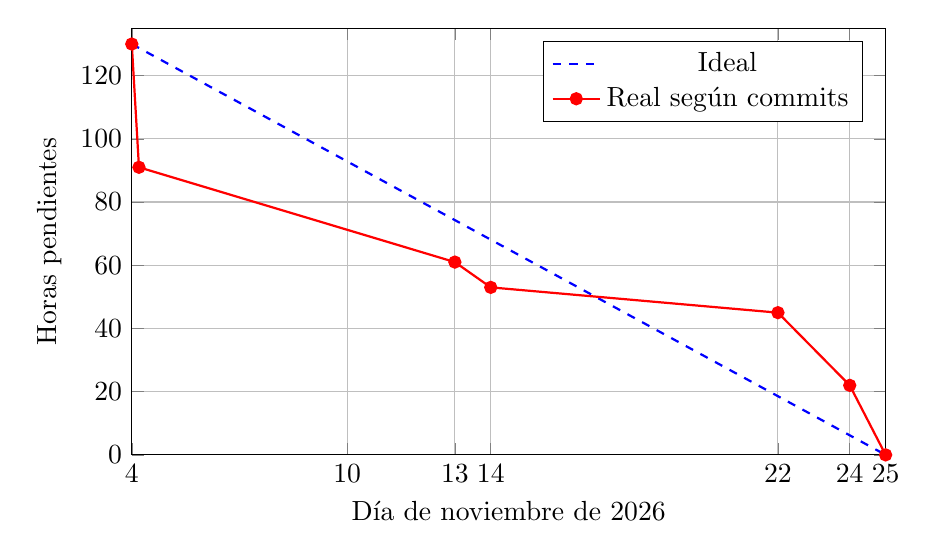
\begin{tikzpicture}
\begin{axis}[width=0.92\textwidth,height=7cm,xmin=4,xmax=25,ymin=0,ymax=135,xtick={4,10,13,14,22,24,25},xlabel={Día de noviembre de 2026},ylabel={Horas pendientes},grid=major,legend pos=north east]
\addplot[blue,dashed,thick] coordinates {(4,130)(25,0)};\addlegendentry{Ideal}
\addplot[red,mark=*,thick] coordinates {(4,130)(4.2,91)(13,61)(14,53)(22,45)(24,22)(25,0)};\addlegendentry{Real según commits}
\end{axis}
\end{tikzpicture}
\caption{Burndown reconstruido con las fechas de los commits del Sprint 3}
\end{figure}

\subsection{Riesgos y mitigación}
\begin{itemize}
\item El cambio de regla conversado con el docente podía afectar análisis y decisiones. Se separó el bloqueo por créditos de la recomendación por contenidos y se reflejó en pruebas y textos.
\item La IA local Ollama podía tardar o no estar disponible. Se añadió reintento automático y un estado comprensible para la solicitud.
\item El trabajo en ramas paralelas podía causar diferencias de integración. Se corrigieron contratos, migraciones y pruebas de integración antes del cierre.
\item Los datos de prueba podían no representar certificados reales. Se prepararon certificados SIHA de ejemplo, casos con errores y pruebas manuales por rol.
\end{itemize}

\subsection{Criterios de finalización}
El sprint se considera terminado cuando el certificado se valida antes de registrarse, el análisis presenta su recomendación por materia, los dos docentes pueden votar, un desacuerdo requiere decisión motivada del administrador, los resultados quedan disponibles por materia y el registro manual aplica controles equivalentes. También se consideran las pruebas automáticas, la ronda manual documentada en la sección 10 y los hallazgos pendientes explícitos.
